\chapter{Durchführung}
Im Versuch werden die zuvor vorgestellten Schwingkreise vermessen. Dazu werden zwei Verfahren angewandt. Im ersten führen wir die Messung mit einem Analogen Oszilloskop durch. Dazu werden im Oszilloskop die Spannungen $U_x$ und $U_y$ aus \figref{fig:aufbau_analog_messung} gegeneinander aufgetragen. Die gegeneinander verschobenen Oszillationen der Spannungen erzeugen auf dem Bildschirm des Oszilloskops Lissajous-Figuren. Die Halbachsen der Ellipsen sowie die Verstärkungsverhältnisse am Oszilloskop ermöglichen zusammen mit der Kenntnis des Widerstands $R_\text{gr}$ eine Bestimmung der Impedanz des Schwingkreises.
\begin{align*}
    |Z|&=R_\text{gr}\,\frac{p_x}{p_y}\\
    \tan\frac{\varphi}{2}&=\frac{b}{a}
\end{align*}
$p_x$ und $p_y$ bezeichnen hier die Verstärkungsfaktoren für die Achsen des Oszilloskops. $a$ und $b$ sind die große und kleine Halbachse der Lissajous-Figur. Eine genaue Herleitung dieser Beziehungen wurde in der Anleitung zur Verfügung gestellt.\\\\
Im zweiten Teil des Experiments wurden die Schwingkreise mit Hilfe von Cassy vermessen. Eines der Cassy-Module stellte dazu die externe Spannung für die Schwingkreise zur Verfügung, während ein anderes wieder die Spannungen $U_x$ und $U_y$ aus \figref{fig:aufbau_analog_messung} aufzeichnete. Zur Berechnung der Impedanz und anderer elektrischer Größen wurde ein vorgefertigtes Cassy-Programm zur Verfügung gestellt.

\begin{figure}[H]
    \centering
    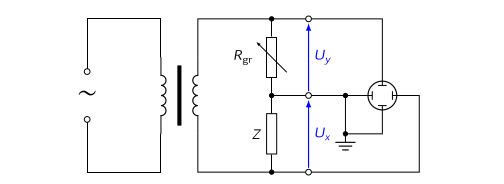
\includegraphics[width = \textwidth]{pictures/messung_analog_re.png}
    \caption{\textbf{Aufbau der Messschaltung.} Der Widerstand $R_\text{gr}$ wird für die analoge Messung so eingestellt, dass die Lissajous-Figur auf auf dem Rand eines Quadrats im Oszilloskop erscheint.}
    \label{fig:aufbau_analog_messung}
\end{figure}
\vfill